\begin{center}
    \begin{figure}[H]
        \centering

        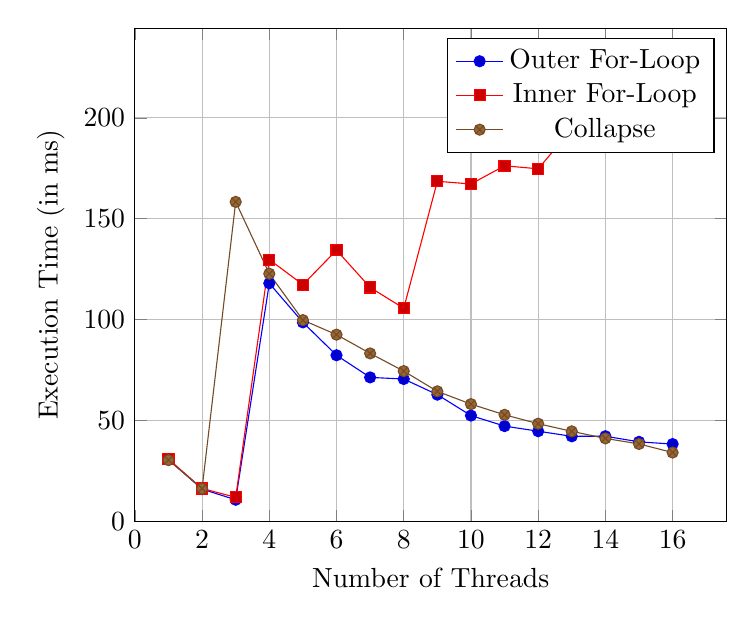
\begin{tikzpicture}
            \begin{axis}[
                title={},
                width=0.75\textwidth,
                xlabel={Number of Threads},
                ylabel={Execution Time (in ms)},
                xmin=0,
                ymin=0,
                grid=major
            ]
                \addplot coordinates {
                    (1,30.641)(2,15.9525)(3,10.6776)(4,117.995)(5,98.6225)(6,82.324)(7,71.3444)(8,70.5416)(9,62.7889)(10,52.4211)(11,47.1942)(12,44.6635)(13,42.1298)(14,42.1888)(15,39.3924)(16,38.2957)
                };
                \addlegendentry{Outer For-Loop}

                \addplot coordinates {
                    (1,30.7855)(2,16.2723)(3,11.8813)(4,129.745)(5,117.341)(6,134.39)(7,115.95)(8,105.581)(9,168.57)(10,167.237)(11,176.252)(12,174.76)(13,194.364)(14,216.556)(15,222.227)(16,216.753)
                };
                \addlegendentry{Inner For-Loop}       

                \addplot coordinates {
                    (1,30.3377)(2,16.2134)(3,158.358)(4,122.745)(5,99.7314)(6,92.5357)(7,83.2476)(8,74.4663)(9,64.432)(10,58.0962)(11,52.7946)(12,48.3936)(13,44.5975)(14,41.1037)(15,38.3576)(16,34.0934)
                };
                \addlegendentry{Collapse}
            \end{axis}
        \end{tikzpicture}
        \caption{Emboss Performance Tests dice.png}
    \end{figure}
\end{center}